\refstepcounter{section}
\section*{Lecture 25: Introduction to Cosmology}
\addcontentsline{toc}{section}{Lecture 25: Introduction to Cosmology}
Cosmology literally means the study of the \textit{cosmos} (`Universe') and is one of the oldest subjects studied by humans. Cosmology, as a philosophy, have been prevalent since prehistoric times. Stars and other heavenly objects have been demonstrated in cave paintings and other evidences of ancient life. \\[0.2cm]
Almost every civilisation have studied cosmology in some form or the other. The concept of Brahmanda goes way back to the Vedic age and describes the creation of the Universe from a `cosmic egg'. \\[0.2cm]
Keeping aside the philosophical and religious aspects of Cosmology (which might land us in controversis), we will mostly discuss about \textit{physical cosmology}, which is the study of cosmological models, defined with respect to measurable physical quantitites like size, density, etc. 
\subsection{The scale and the physics}
Imagine a glass of water. To measure the density of the water, we can take any mass of water from the glass and then measure the volume. Dividing the mass by the volume we get the density. We find it to be approximately $1\ \mathrm{g}/\mathrm{cc}$ and we can fairly estimate that the glass of water is homogenous and at each point the density will be the same. We can take as much small quantity of water for measurement as possible with our everyday apparatus.\\[0.2cm] However, if we use say some electron microscope to resolve between the molecules of water and in some divine way, use this to measure the density, we would find that the density does not remain fix. In fact, at this length scale $\sim10^{-10}$ m the concept of density doesn't make much sense. 
\begin{figure}[H]
  \centering
    

\tikzset{every picture/.style={line width=0.75pt}} %set default line width to 0.75pt        

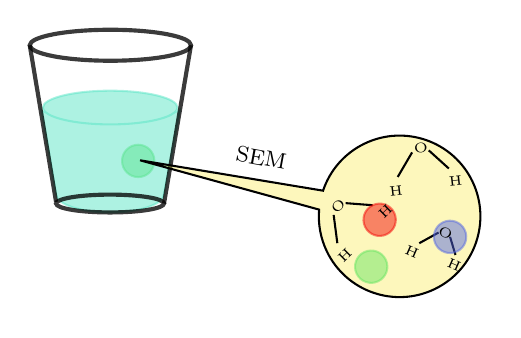
\begin{tikzpicture}[x=0.75pt,y=0.75pt,yscale=-1,xscale=1]
%uncomment if require: \path (0,300); %set diagram left start at 0, and has height of 300

%Shape: Circle [id:dp7684119478579371] 
\draw  [color={rgb, 255:red, 98; green, 228; blue, 96 }  ,draw opacity=0.47 ][fill={rgb, 255:red, 98; green, 228; blue, 96 }  ,fill opacity=0.47 ] (267.46,104.19) .. controls (267.46,99.89) and (270.95,96.4) .. (275.25,96.4) .. controls (279.55,96.4) and (283.04,99.89) .. (283.04,104.19) .. controls (283.04,108.49) and (279.55,111.98) .. (275.25,111.98) .. controls (270.95,111.98) and (267.46,108.49) .. (267.46,104.19) -- cycle ;
%Shape: Path Data [id:dp25808855703671085] 
\draw  [color={rgb, 255:red, 80; green, 227; blue, 194 }  ,draw opacity=0.47 ][fill={rgb, 255:red, 80; green, 227; blue, 194 }  ,fill opacity=0.47 ] (287.68,120.12) .. controls (287.68,125.03) and (276.04,129.02) .. (261.68,129.02) .. controls (247.32,129.02) and (235.68,125.03) .. (235.68,120.12) -- (228.81,79.84) .. controls (229.38,80.14) and (229.96,80.43) .. (230.57,80.71) .. controls (229.77,80) and (229.34,79.25) .. (229.34,78.48) .. controls (229.34,74) and (243.86,70.36) .. (261.76,70.36) .. controls (279.67,70.36) and (294.18,74) .. (294.18,78.48) .. controls (294.18,79.25) and (293.76,80) .. (292.96,80.71) .. controls (293.78,80.32) and (294.58,79.92) .. (295.33,79.51) -- (287.68,120.12) -- cycle (230.57,80.71) .. controls (234.43,84.11) and (246.93,86.61) .. (261.76,86.61) .. controls (276.59,86.61) and (289.1,84.11) .. (292.96,80.71) -- (292.96,80.71) .. controls (289.1,84.11) and (276.59,86.61) .. (261.76,86.61) .. controls (246.93,86.61) and (234.43,84.11) .. (230.57,80.71) -- cycle ;
%Shape: Ellipse [id:dp16082097522679295] 
\draw  [color={rgb, 255:red, 0; green, 0; blue, 0 }  ,draw opacity=0.77 ][line width=1.5]  (223,48.47) .. controls (223,44.34) and (240.39,41) .. (261.84,41) .. controls (283.29,41) and (300.68,44.34) .. (300.68,48.47) .. controls (300.68,52.59) and (283.29,55.93) .. (261.84,55.93) .. controls (240.39,55.93) and (223,52.59) .. (223,48.47) -- cycle ;
%Straight Lines [id:da37253082195391385] 
\draw [color={rgb, 255:red, 0; green, 0; blue, 0 }  ,draw opacity=0.77 ][line width=1.5]    (223,48.47) -- (235.68,123.93) ;
%Straight Lines [id:da3601617754801465] 
\draw [color={rgb, 255:red, 0; green, 0; blue, 0 }  ,draw opacity=0.77 ][line width=1.5]    (300.68,48.47) -- (287.68,124.72) ;
%Shape: Ellipse [id:dp9629053055122511] 
\draw  [color={rgb, 255:red, 0; green, 0; blue, 0 }  ,draw opacity=0.77 ][line width=1.5]  (235.68,124.72) .. controls (235.68,122.35) and (247.32,120.43) .. (261.68,120.43) .. controls (276.04,120.43) and (287.68,122.35) .. (287.68,124.72) .. controls (287.68,127.1) and (276.04,129.02) .. (261.68,129.02) .. controls (247.32,129.02) and (235.68,127.1) .. (235.68,124.72) -- cycle ;

%Shape: Path Data [id:dp8985709510975483] 
\draw  [fill={rgb, 255:red, 248; green, 232; blue, 51 }  ,fill opacity=0.33 ] (384.27,95.87) .. controls (403.61,86.52) and (426.88,94.63) .. (436.23,113.97) .. controls (445.58,133.32) and (437.47,156.59) .. (418.12,165.93) .. controls (398.77,175.28) and (375.51,167.18) .. (366.16,147.83) .. controls (363.02,141.32) and (361.85,134.37) .. (362.42,127.66) -- (276.15,103.9) -- (364.31,118.53) .. controls (367.52,108.94) and (374.45,100.61) .. (384.27,95.87) -- cycle ;
%Straight Lines [id:da18060147064064824] 
\draw    (369.42,130.22) -- (371.19,143.83) ;
%Straight Lines [id:da8994922446338276] 
\draw    (388.19,125.53) -- (375.2,124.54) ;
%Straight Lines [id:da4313587615843497] 
\draw    (419.96,138.71) -- (410.66,143.85) ;
%Straight Lines [id:da031098467049276324] 
\draw    (428.11,149.51) -- (425.5,140.79) ;
%Straight Lines [id:da40090968151420037] 
\draw    (407.21,100.09) -- (400.28,111.93) ;
%Straight Lines [id:da631678586008194] 
\draw    (424.92,107.87) -- (415.26,99.13) ;
%Shape: Circle [id:dp7327796708226236] 
\draw  [color={rgb, 255:red, 98; green, 228; blue, 96 }  ,draw opacity=0.47 ][fill={rgb, 255:red, 98; green, 228; blue, 96 }  ,fill opacity=0.47 ] (380.49,158.55) .. controls (378.61,154.67) and (380.24,150.02) .. (384.11,148.14) .. controls (387.99,146.27) and (392.64,147.89) .. (394.52,151.77) .. controls (396.39,155.64) and (394.77,160.3) .. (390.89,162.17) .. controls (387.02,164.05) and (382.36,162.42) .. (380.49,158.55) -- cycle ;
%Shape: Circle [id:dp8847449751952173] 
\draw  [color={rgb, 255:red, 81; green, 100; blue, 226 }  ,draw opacity=0.47 ][fill={rgb, 255:red, 81; green, 100; blue, 226 }  ,fill opacity=0.47 ] (418.48,144.18) .. controls (416.61,140.3) and (418.24,135.64) .. (422.11,133.77) .. controls (425.99,131.9) and (430.64,133.52) .. (432.52,137.4) .. controls (434.39,141.27) and (432.76,145.93) .. (428.89,147.8) .. controls (425.02,149.67) and (420.36,148.05) .. (418.48,144.18) -- cycle ;
%Shape: Circle [id:dp4111104283157898] 
\draw  [color={rgb, 255:red, 243; green, 5; blue, 5 }  ,draw opacity=0.48 ][fill={rgb, 255:red, 243; green, 5; blue, 5 }  ,fill opacity=0.48 ] (384.56,135.93) .. controls (382.69,132.06) and (384.31,127.4) .. (388.19,125.53) .. controls (392.06,123.66) and (396.72,125.28) .. (398.59,129.15) .. controls (400.46,133.03) and (398.84,137.69) .. (394.97,139.56) .. controls (391.09,141.43) and (386.43,139.81) .. (384.56,135.93) -- cycle ;

% Text Node
\draw (322.09,95.14) node [anchor=north west][inner sep=0.75pt]  [font=\footnotesize,rotate=-10.51] [align=left] {SEM};
% Text Node
\draw (365.39,126.79) node [anchor=north west][inner sep=0.75pt]  [font=\tiny,rotate=-315.47] [align=left] {O};
% Text Node
\draw (368.76,150.46) node [anchor=north west][inner sep=0.75pt]  [font=\tiny,rotate=-315.47] [align=left] {H};
% Text Node
\draw (388.34,128.94) node [anchor=north west][inner sep=0.75pt]  [font=\tiny,rotate=-315.47] [align=left] {H};
% Text Node
\draw (420.35,133.41) node [anchor=north west][inner sep=0.75pt]  [font=\tiny,rotate=-23.56] [align=left] {O};
% Text Node
\draw (404.25,142.55) node [anchor=north west][inner sep=0.75pt]  [font=\tiny,rotate=-23.56] [align=left] {H};
% Text Node
\draw (424.67,148.94) node [anchor=north west][inner sep=0.75pt]  [font=\tiny,rotate=-23.56] [align=left] {H};
% Text Node
\draw (406.13,94.9) node [anchor=north west][inner sep=0.75pt]  [font=\tiny,rotate=-353.23] [align=left] {O};
% Text Node
\draw (394.29,115.68) node [anchor=north west][inner sep=0.75pt]  [font=\tiny,rotate=-353.23] [align=left] {H};
% Text Node
\draw (422.95,110.66) node [anchor=north west][inner sep=0.75pt]  [font=\tiny,rotate=-353.23] [align=left] {H};


\end{tikzpicture}

\end{figure}
% \begin{figure}[H]
%     \centering
%     

\tikzset{every picture/.style={line width=0.75pt}} %set default line width to 0.75pt        

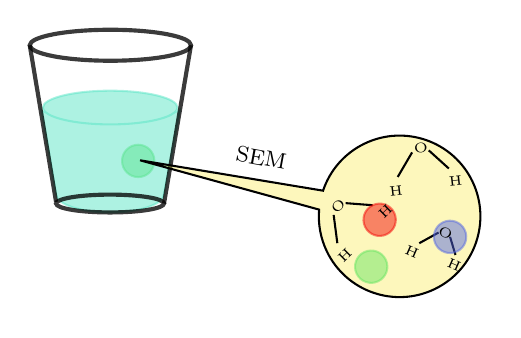
\begin{tikzpicture}[x=0.75pt,y=0.75pt,yscale=-1,xscale=1]
%uncomment if require: \path (0,300); %set diagram left start at 0, and has height of 300

%Shape: Circle [id:dp7684119478579371] 
\draw  [color={rgb, 255:red, 98; green, 228; blue, 96 }  ,draw opacity=0.47 ][fill={rgb, 255:red, 98; green, 228; blue, 96 }  ,fill opacity=0.47 ] (267.46,104.19) .. controls (267.46,99.89) and (270.95,96.4) .. (275.25,96.4) .. controls (279.55,96.4) and (283.04,99.89) .. (283.04,104.19) .. controls (283.04,108.49) and (279.55,111.98) .. (275.25,111.98) .. controls (270.95,111.98) and (267.46,108.49) .. (267.46,104.19) -- cycle ;
%Shape: Path Data [id:dp25808855703671085] 
\draw  [color={rgb, 255:red, 80; green, 227; blue, 194 }  ,draw opacity=0.47 ][fill={rgb, 255:red, 80; green, 227; blue, 194 }  ,fill opacity=0.47 ] (287.68,120.12) .. controls (287.68,125.03) and (276.04,129.02) .. (261.68,129.02) .. controls (247.32,129.02) and (235.68,125.03) .. (235.68,120.12) -- (228.81,79.84) .. controls (229.38,80.14) and (229.96,80.43) .. (230.57,80.71) .. controls (229.77,80) and (229.34,79.25) .. (229.34,78.48) .. controls (229.34,74) and (243.86,70.36) .. (261.76,70.36) .. controls (279.67,70.36) and (294.18,74) .. (294.18,78.48) .. controls (294.18,79.25) and (293.76,80) .. (292.96,80.71) .. controls (293.78,80.32) and (294.58,79.92) .. (295.33,79.51) -- (287.68,120.12) -- cycle (230.57,80.71) .. controls (234.43,84.11) and (246.93,86.61) .. (261.76,86.61) .. controls (276.59,86.61) and (289.1,84.11) .. (292.96,80.71) -- (292.96,80.71) .. controls (289.1,84.11) and (276.59,86.61) .. (261.76,86.61) .. controls (246.93,86.61) and (234.43,84.11) .. (230.57,80.71) -- cycle ;
%Shape: Ellipse [id:dp16082097522679295] 
\draw  [color={rgb, 255:red, 0; green, 0; blue, 0 }  ,draw opacity=0.77 ][line width=1.5]  (223,48.47) .. controls (223,44.34) and (240.39,41) .. (261.84,41) .. controls (283.29,41) and (300.68,44.34) .. (300.68,48.47) .. controls (300.68,52.59) and (283.29,55.93) .. (261.84,55.93) .. controls (240.39,55.93) and (223,52.59) .. (223,48.47) -- cycle ;
%Straight Lines [id:da37253082195391385] 
\draw [color={rgb, 255:red, 0; green, 0; blue, 0 }  ,draw opacity=0.77 ][line width=1.5]    (223,48.47) -- (235.68,123.93) ;
%Straight Lines [id:da3601617754801465] 
\draw [color={rgb, 255:red, 0; green, 0; blue, 0 }  ,draw opacity=0.77 ][line width=1.5]    (300.68,48.47) -- (287.68,124.72) ;
%Shape: Ellipse [id:dp9629053055122511] 
\draw  [color={rgb, 255:red, 0; green, 0; blue, 0 }  ,draw opacity=0.77 ][line width=1.5]  (235.68,124.72) .. controls (235.68,122.35) and (247.32,120.43) .. (261.68,120.43) .. controls (276.04,120.43) and (287.68,122.35) .. (287.68,124.72) .. controls (287.68,127.1) and (276.04,129.02) .. (261.68,129.02) .. controls (247.32,129.02) and (235.68,127.1) .. (235.68,124.72) -- cycle ;

%Shape: Path Data [id:dp8985709510975483] 
\draw  [fill={rgb, 255:red, 248; green, 232; blue, 51 }  ,fill opacity=0.33 ] (384.27,95.87) .. controls (403.61,86.52) and (426.88,94.63) .. (436.23,113.97) .. controls (445.58,133.32) and (437.47,156.59) .. (418.12,165.93) .. controls (398.77,175.28) and (375.51,167.18) .. (366.16,147.83) .. controls (363.02,141.32) and (361.85,134.37) .. (362.42,127.66) -- (276.15,103.9) -- (364.31,118.53) .. controls (367.52,108.94) and (374.45,100.61) .. (384.27,95.87) -- cycle ;
%Straight Lines [id:da18060147064064824] 
\draw    (369.42,130.22) -- (371.19,143.83) ;
%Straight Lines [id:da8994922446338276] 
\draw    (388.19,125.53) -- (375.2,124.54) ;
%Straight Lines [id:da4313587615843497] 
\draw    (419.96,138.71) -- (410.66,143.85) ;
%Straight Lines [id:da031098467049276324] 
\draw    (428.11,149.51) -- (425.5,140.79) ;
%Straight Lines [id:da40090968151420037] 
\draw    (407.21,100.09) -- (400.28,111.93) ;
%Straight Lines [id:da631678586008194] 
\draw    (424.92,107.87) -- (415.26,99.13) ;
%Shape: Circle [id:dp7327796708226236] 
\draw  [color={rgb, 255:red, 98; green, 228; blue, 96 }  ,draw opacity=0.47 ][fill={rgb, 255:red, 98; green, 228; blue, 96 }  ,fill opacity=0.47 ] (380.49,158.55) .. controls (378.61,154.67) and (380.24,150.02) .. (384.11,148.14) .. controls (387.99,146.27) and (392.64,147.89) .. (394.52,151.77) .. controls (396.39,155.64) and (394.77,160.3) .. (390.89,162.17) .. controls (387.02,164.05) and (382.36,162.42) .. (380.49,158.55) -- cycle ;
%Shape: Circle [id:dp8847449751952173] 
\draw  [color={rgb, 255:red, 81; green, 100; blue, 226 }  ,draw opacity=0.47 ][fill={rgb, 255:red, 81; green, 100; blue, 226 }  ,fill opacity=0.47 ] (418.48,144.18) .. controls (416.61,140.3) and (418.24,135.64) .. (422.11,133.77) .. controls (425.99,131.9) and (430.64,133.52) .. (432.52,137.4) .. controls (434.39,141.27) and (432.76,145.93) .. (428.89,147.8) .. controls (425.02,149.67) and (420.36,148.05) .. (418.48,144.18) -- cycle ;
%Shape: Circle [id:dp4111104283157898] 
\draw  [color={rgb, 255:red, 243; green, 5; blue, 5 }  ,draw opacity=0.48 ][fill={rgb, 255:red, 243; green, 5; blue, 5 }  ,fill opacity=0.48 ] (384.56,135.93) .. controls (382.69,132.06) and (384.31,127.4) .. (388.19,125.53) .. controls (392.06,123.66) and (396.72,125.28) .. (398.59,129.15) .. controls (400.46,133.03) and (398.84,137.69) .. (394.97,139.56) .. controls (391.09,141.43) and (386.43,139.81) .. (384.56,135.93) -- cycle ;

% Text Node
\draw (322.09,95.14) node [anchor=north west][inner sep=0.75pt]  [font=\footnotesize,rotate=-10.51] [align=left] {SEM};
% Text Node
\draw (365.39,126.79) node [anchor=north west][inner sep=0.75pt]  [font=\tiny,rotate=-315.47] [align=left] {O};
% Text Node
\draw (368.76,150.46) node [anchor=north west][inner sep=0.75pt]  [font=\tiny,rotate=-315.47] [align=left] {H};
% Text Node
\draw (388.34,128.94) node [anchor=north west][inner sep=0.75pt]  [font=\tiny,rotate=-315.47] [align=left] {H};
% Text Node
\draw (420.35,133.41) node [anchor=north west][inner sep=0.75pt]  [font=\tiny,rotate=-23.56] [align=left] {O};
% Text Node
\draw (404.25,142.55) node [anchor=north west][inner sep=0.75pt]  [font=\tiny,rotate=-23.56] [align=left] {H};
% Text Node
\draw (424.67,148.94) node [anchor=north west][inner sep=0.75pt]  [font=\tiny,rotate=-23.56] [align=left] {H};
% Text Node
\draw (406.13,94.9) node [anchor=north west][inner sep=0.75pt]  [font=\tiny,rotate=-353.23] [align=left] {O};
% Text Node
\draw (394.29,115.68) node [anchor=north west][inner sep=0.75pt]  [font=\tiny,rotate=-353.23] [align=left] {H};
% Text Node
\draw (422.95,110.66) node [anchor=north west][inner sep=0.75pt]  [font=\tiny,rotate=-353.23] [align=left] {H};


\end{tikzpicture}

% \end{figure}
\noindent
In the figure, we find that on a coarse-grained scale, the entire glass of water looks homogenous with almost constant density (statistical fluctuations are always there). However, on zooming a particular region upto the atomic scale, we find that the constituents in the red, green and blue regions are totally different and the concept of homogenity becomes invalid. \\[0.2cm]
We note that there is a difference of $8 orders$ between the coarse-grained $\mathrm{cm}$ length scale when homogenity is there and the $\mathrm{atomic}$ length scale where there is no homogenity.\\[0.2cm]
So one must apply different physical concepts at different scales, even to study the same system \emoji{exploding-head}! The same thing happens to our Universe also where based on different length scales, the Universe looks different. 
\begin{figure}[H]
    \centering 
    

% Gradient Info
  
\tikzset {_m31uq9hnc/.code = {\pgfsetadditionalshadetransform{ \pgftransformshift{\pgfpoint{0 bp } { 0 bp }  }  \pgftransformrotate{0 }  \pgftransformscale{2 }  }}}
\pgfdeclarehorizontalshading{_ja0yc92wl}{150bp}{rgb(0bp)=(0.94,0.98,1);
rgb(37.5bp)=(0.94,0.98,1);
rgb(47.385417393275674bp)=(0.8,0.92,1);
rgb(62.5bp)=(0.63,0.86,1);
rgb(100bp)=(0.63,0.86,1)}

% Pattern Info
 
\tikzset{
pattern size/.store in=\mcSize, 
pattern size = 5pt,
pattern thickness/.store in=\mcThickness, 
pattern thickness = 0.3pt,
pattern radius/.store in=\mcRadius, 
pattern radius = 1pt}
\makeatletter
\pgfutil@ifundefined{pgf@pattern@name@_3lru2hhbp}{
\makeatletter
\pgfdeclarepatternformonly[\mcRadius,\mcThickness,\mcSize]{_3lru2hhbp}
{\pgfpoint{-0.5*\mcSize}{-0.5*\mcSize}}
{\pgfpoint{0.5*\mcSize}{0.5*\mcSize}}
{\pgfpoint{\mcSize}{\mcSize}}
{
\pgfsetcolor{\tikz@pattern@color}
\pgfsetlinewidth{\mcThickness}
\pgfpathcircle\pgfpointorigin{\mcRadius}
\pgfusepath{stroke}
}}
\makeatother

% Gradient Info
  
\tikzset {_pq0hm2nsf/.code = {\pgfsetadditionalshadetransform{ \pgftransformshift{\pgfpoint{0 bp } { 0 bp }  }  \pgftransformrotate{0 }  \pgftransformscale{2 }  }}}
\pgfdeclarehorizontalshading{_0zassn5ur}{150bp}{rgb(0bp)=(1,0.84,0.37);
rgb(37.5bp)=(1,0.84,0.37);
rgb(62.5bp)=(1,0.75,0.02);
rgb(100bp)=(1,0.75,0.02)}
\tikzset{every picture/.style={line width=0.75pt}} %set default line width to 0.75pt        

\begin{tikzpicture}[x=0.75pt,y=0.75pt,yscale=-1,xscale=1]
%uncomment if require: \path (0,418); %set diagram left start at 0, and has height of 418

%Shape: Spiral [id:dp5394210484770013] 
\draw   (375.92,96.51) .. controls (376.66,96.72) and (377.22,96.92) .. (377.68,97.12) .. controls (378.14,97.34) and (378.22,97.44) .. (377.88,97.46) .. controls (377.59,97.48) and (376.8,97.35) .. (375.76,97.13) .. controls (374.55,96.87) and (373.19,96.52) .. (371.62,96.06) .. controls (369.84,95.54) and (368.32,95.03) .. (366.88,94.49) .. controls (365.32,93.9) and (364.21,93.4) .. (363.58,93) .. controls (362.89,92.55) and (362.96,92.31) .. (363.65,92.24) .. controls (364.44,92.17) and (365.95,92.35) .. (368.09,92.74) .. controls (370.38,93.15) and (373.2,93.81) .. (376.43,94.65) .. controls (379.87,95.55) and (383.32,96.56) .. (386.69,97.65) .. controls (390.27,98.81) and (393.38,99.93) .. (395.82,100.96) .. controls (398.49,102.06) and (400.02,102.91) .. (400.6,103.54) .. controls (401.22,104.2) and (400.61,104.52) .. (398.71,104.45) .. controls (396.72,104.38) and (393.74,103.94) .. (389.64,103.12) .. controls (385.3,102.24) and (380.54,101.09) .. (375.08,99.61) .. controls (369.46,98.09) and (364,96.45) .. (358.69,94.69) .. controls (353.18,92.86) and (348.67,91.18) .. (345.17,89.64) .. controls (341.55,88.05) and (339.41,86.81) .. (338.91,85.97) .. controls (338.33,85.07) and (339.66,84.74) .. (342.62,84.91) .. controls (345.77,85.1) and (350.33,85.82) .. (356.33,87.07) .. controls (362.57,88.38) and (369.46,90.07) .. (377.1,92.17) .. controls (384.96,94.33) and (392.42,96.6) .. (399.61,99.02) .. controls (407.02,101.51) and (412.93,103.75) .. (417.53,105.8) .. controls (422.25,107.92) and (424.82,109.5) .. (425.28,110.57) .. controls (425.78,111.68) and (423.91,112.08) .. (419.75,111.78) .. controls (415.49,111.47) and (409.35,110.47) .. (401.4,108.78) .. controls (393.21,107.04) and (384.19,104.8) .. (374.41,102.09) .. controls (364.36,99.31) and (354.81,96.38) .. (345.77,93.32) .. controls (336.52,90.19) and (329.12,87.36) .. (323.46,84.8) .. controls (317.69,82.18) and (314.6,80.23) .. (314.23,78.94) .. controls (313.86,77.62) and (316.26,77.16) .. (321.58,77.58) .. controls (327,78.01) and (334.62,79.28) .. (344.57,81.41) .. controls (354.67,83.58) and (365.72,86.33) .. (377.78,89.69) .. controls (390.05,93.11) and (401.61,96.67) .. (412.54,100.39) .. controls (423.68,104.18) and (432.58,107.6) .. (439.24,110.65) .. controls (446.01,113.76) and (449.62,116.09) .. (449.96,117.6) .. controls (450.34,119.15) and (447.21,119.64) .. (440.78,119.11) .. controls (434.16,118.55) and (424.96,117) .. (413.15,114.44) .. controls (401.11,111.85) and (387.93,108.54) .. (373.74,104.57) .. controls (359.27,100.53) and (345.62,96.32) .. (332.85,91.95) .. controls (319.87,87.52) and (309.47,83.51) .. (301.75,79.95) .. controls (293.93,76.33) and (289.8,73.64) .. (289.55,71.91) .. controls (289.3,70.15) and (292.96,69.6) .. (300.55,70.25) .. controls (308.23,70.92) and (319.01,72.75) .. (332.82,75.75) .. controls (346.76,78.77) and (362.07,82.62) .. (378.45,87.21) .. controls (395.15,91.89) and (410.8,96.73) .. (425.46,101.75) .. controls (440.34,106.84) and (452.13,111.42) .. (460.95,115.5) .. controls (469.87,119.63) and (474.43,122.68) .. (474.64,124.63) .. controls (474.91,126.63) and (470.61,127.22) .. (461.82,126.43) .. controls (452.93,125.64) and (440.67,123.54) .. (424.91,120.11) .. controls (409.02,116.65) and (391.68,112.28) .. (373.06,107.05) .. controls (354.18,101.75) and (336.43,96.25) .. (319.93,90.59) .. controls (303.21,84.85) and (289.92,79.68) .. (280.04,75.1) .. controls (270.07,70.46) and (265,67.04) .. (264.87,64.88) .. controls (264.73,62.67) and (269.57,62.01) .. (279.51,62.93) .. controls (289.56,63.84) and (303.4,66.22) .. (321.06,70.09) .. controls (338.95,74) and (358.32,78.88) .. (379.12,84.73) .. controls (400.24,90.67) and (419.99,96.8) .. (438.38,103.12) .. controls (457,109.52) and (471.78,115.27) .. (482.66,120.35) .. controls (493.64,125.48) and (499.23,129.26) .. (499.32,131.66) .. controls (499.32,131.66) and (499.32,131.66) .. (499.32,131.66) ;
%Shape: Path Data [id:dp6172560893603736] 
\path  [shading=_ja0yc92wl,_m31uq9hnc] (269.36,162.43) .. controls (329.03,162.43) and (377.4,179.13) .. (377.4,199.74) .. controls (377.4,220.34) and (329.03,237.04) .. (269.36,237.04) .. controls (209.69,237.04) and (161.31,220.34) .. (161.31,199.74) .. controls (161.31,179.13) and (209.69,162.43) .. (269.36,162.43) -- cycle ; % for fading 
 \draw  [dash pattern={on 4.5pt off 4.5pt}] (269.36,162.43) .. controls (329.03,162.43) and (377.4,179.13) .. (377.4,199.74) .. controls (377.4,220.34) and (329.03,237.04) .. (269.36,237.04) .. controls (209.69,237.04) and (161.31,220.34) .. (161.31,199.74) .. controls (161.31,179.13) and (209.69,162.43) .. (269.36,162.43) -- cycle ; % for border 

%Shape: Path Data [id:dp24624210108482714] 
\draw  [draw opacity=0][pattern=_3lru2hhbp,pattern size=6pt,pattern thickness=0.75pt,pattern radius=0.75pt, pattern color={rgb, 255:red, 0; green, 0; blue, 0}][dash pattern={on 4.5pt off 4.5pt}] (269.36,162.43) .. controls (329.03,162.43) and (377.4,179.13) .. (377.4,199.74) .. controls (377.4,220.34) and (329.03,237.04) .. (269.36,237.04) .. controls (209.69,237.04) and (161.31,220.34) .. (161.31,199.74) .. controls (161.31,179.13) and (209.69,162.43) .. (269.36,162.43) -- cycle ;

%Shape: Ellipse [id:dp3698488797345263] 
\draw  [color={rgb, 255:red, 255; green, 0; blue, 0 }  ,draw opacity=1 ][fill={rgb, 255:red, 255; green, 0; blue, 0 }  ,fill opacity=1 ] (265.22,201.19) .. controls (265.22,200.21) and (266,199.42) .. (266.95,199.42) .. controls (267.91,199.42) and (268.68,200.21) .. (268.68,201.19) .. controls (268.68,202.17) and (267.91,202.96) .. (266.95,202.96) .. controls (266,202.96) and (265.22,202.17) .. (265.22,201.19) -- cycle ;
%Shape: Ellipse [id:dp0525399008633608] 
\draw  [color={rgb, 255:red, 255; green, 0; blue, 0 }  ,draw opacity=1 ][fill={rgb, 255:red, 255; green, 0; blue, 0 }  ,fill opacity=1 ] (341.26,91.41) .. controls (341.64,90.52) and (342.66,90.11) .. (343.53,90.5) .. controls (344.41,90.89) and (344.81,91.93) .. (344.43,92.83) .. controls (344.05,93.72) and (343.03,94.13) .. (342.15,93.74) .. controls (341.28,93.35) and (340.88,92.31) .. (341.26,91.41) -- cycle ;
%Shape: Path Data [id:dp1707870930498112] 
\draw  [fill={rgb, 255:red, 255; green, 255; blue, 255 }  ,fill opacity=1 ] (266.95,201.19) -- (340.42,114.83) -- (334.61,110.02) -- (354.05,107.53) -- (355.77,127.52) -- (349.74,122.54) -- (266.95,201.19) -- cycle ;
%Shape: Path Data [id:dp1949318860064807] 
\draw  [fill={rgb, 255:red, 255; green, 255; blue, 255 }  ,fill opacity=1 ] (335.39,89.94) -- (196.41,97.05) -- (196.88,106.5) -- (178.52,90.86) -- (195.16,72.09) -- (195.65,81.89) -- (335.39,89.94) -- cycle ;
%Shape: Ellipse [id:dp2904507110095169] 
\path  [shading=_0zassn5ur,_pq0hm2nsf] (105.38,81.98) .. controls (105.38,76.48) and (109.74,72.02) .. (115.11,72.02) .. controls (120.49,72.02) and (124.84,76.48) .. (124.84,81.98) .. controls (124.84,87.49) and (120.49,91.95) .. (115.11,91.95) .. controls (109.74,91.95) and (105.38,87.49) .. (105.38,81.98) -- cycle ; % for fading 
 \draw   (105.38,81.98) .. controls (105.38,76.48) and (109.74,72.02) .. (115.11,72.02) .. controls (120.49,72.02) and (124.84,76.48) .. (124.84,81.98) .. controls (124.84,87.49) and (120.49,91.95) .. (115.11,91.95) .. controls (109.74,91.95) and (105.38,87.49) .. (105.38,81.98) -- cycle ; % for border 

%Straight Lines [id:da3524392246563651] 
\draw  [dash pattern={on 0.84pt off 2.51pt}]  (49.68,152.57) -- (169.07,151.82) ;
\draw [shift={(169.07,151.82)}, rotate = 179.64] [color={rgb, 255:red, 0; green, 0; blue, 0 }  ][line width=0.75]    (0,5.59) -- (0,-5.59)   ;
\draw [shift={(49.68,152.57)}, rotate = 179.64] [color={rgb, 255:red, 0; green, 0; blue, 0 }  ][line width=0.75]    (0,5.59) -- (0,-5.59)   ;
%Shape: Arc [id:dp2083216292800627] 
\draw  [draw opacity=0][dash pattern={on 4.5pt off 4.5pt}] (97.83,54.19) .. controls (102.82,50.93) and (108.75,49.04) .. (115.11,49.04) .. controls (132.88,49.04) and (147.28,63.79) .. (147.28,81.98) .. controls (147.28,100.18) and (132.88,114.93) .. (115.11,114.93) .. controls (110.39,114.93) and (105.9,113.89) .. (101.86,112.01) -- (115.11,81.98) -- cycle ; \draw  [dash pattern={on 4.5pt off 4.5pt}] (97.83,54.19) .. controls (102.82,50.93) and (108.75,49.04) .. (115.11,49.04) .. controls (132.88,49.04) and (147.28,63.79) .. (147.28,81.98) .. controls (147.28,100.18) and (132.88,114.93) .. (115.11,114.93) .. controls (110.39,114.93) and (105.9,113.89) .. (101.86,112.01) ;  
%Shape: Arc [id:dp09520676055458965] 
\draw  [draw opacity=0][dash pattern={on 4.5pt off 4.5pt}] (71.73,54.62) .. controls (80.7,39.73) and (96.78,29.81) .. (115.11,29.81) .. controls (143.25,29.81) and (166.05,53.17) .. (166.05,81.98) .. controls (166.05,110.8) and (143.25,134.16) .. (115.11,134.16) .. controls (102.52,134.16) and (91,129.48) .. (82.11,121.73) -- (115.11,81.98) -- cycle ; \draw  [dash pattern={on 4.5pt off 4.5pt}] (71.73,54.62) .. controls (80.7,39.73) and (96.78,29.81) .. (115.11,29.81) .. controls (143.25,29.81) and (166.05,53.17) .. (166.05,81.98) .. controls (166.05,110.8) and (143.25,134.16) .. (115.11,134.16) .. controls (102.52,134.16) and (91,129.48) .. (82.11,121.73) ;  
%Shape: Ellipse [id:dp20941350154267535] 
\draw  [color={rgb, 255:red, 0; green, 0; blue, 0 }  ,draw opacity=1 ][fill={rgb, 255:red, 74; green, 144; blue, 226 }  ,fill opacity=1 ] (143.8,88.24) .. controls (144.37,86.89) and (145.9,86.27) .. (147.22,86.86) .. controls (148.54,87.44) and (149.15,89.01) .. (148.57,90.36) .. controls (148,91.71) and (146.47,92.33) .. (145.15,91.75) .. controls (143.83,91.16) and (143.22,89.59) .. (143.8,88.24) -- cycle ;
%Straight Lines [id:da5586845823644567] 
\draw  [dash pattern={on 0.84pt off 2.51pt}]  (282.05,39.31) -- (483.97,99.29) ;
\draw [shift={(483.97,99.29)}, rotate = 196.54] [color={rgb, 255:red, 0; green, 0; blue, 0 }  ][line width=0.75]    (0,5.59) -- (0,-5.59)   ;
\draw [shift={(282.05,39.31)}, rotate = 196.54] [color={rgb, 255:red, 0; green, 0; blue, 0 }  ][line width=0.75]    (0,5.59) -- (0,-5.59)   ;
%Straight Lines [id:da49900279999307795] 
\draw  [dash pattern={on 0.84pt off 2.51pt}]  (169.87,249.42) -- (374.19,248.08) ;
\draw [shift={(374.19,248.08)}, rotate = 179.62] [color={rgb, 255:red, 0; green, 0; blue, 0 }  ][line width=0.75]    (0,5.59) -- (0,-5.59)   ;
\draw [shift={(169.87,249.42)}, rotate = 179.62] [color={rgb, 255:red, 0; green, 0; blue, 0 }  ][line width=0.75]    (0,5.59) -- (0,-5.59)   ;

% Text Node
\draw (370.29,49.68) node [anchor=north west][inner sep=0.75pt]  [font=\scriptsize,rotate=-15.46]  {$10^{21} \ \mathrm{m} \ $};
% Text Node
\draw (250.28,256.72) node [anchor=north west][inner sep=0.75pt]  [font=\scriptsize]  {$10^{26} \ \mathrm{m} \ $};
% Text Node
\draw (93.24,157.41) node [anchor=north west][inner sep=0.75pt]  [font=\scriptsize]  {$10^{12} \ \mathrm{m} \ $};


\end{tikzpicture}

    \caption{Different length scales of the Universe}
\end{figure}
\noindent
The solar system, with a diameter roughly of order $10^12$ m, looks fairly inhomogenous to us. In some places, there are planets, while in some other places, some asteroids or something else is present. Moving on to the Milkyway galaxy of size of order $10^21$ m, things become a bit smoother but still inhomogenity persists. For the entire observable Universe with estimated size of order $10^26$ m, we can safely assume it to be homogenous fluid. In fact there is a difference of more than $14$ order between the size of the Solar system (from where all measurements of the Universe are to be done) and the observable Universe. It seems that the Universe is even a better fluid than water!
\begin{itemize}
    \item[$\vartriangleright$] Our Universe at large scales look like a fluid!
    \item[$\vartriangleright$] Only around a small region around us, can we take measurements as we cannot `physically' access all parts of the observable Universe 
\end{itemize}
Unlike the glass of water, we cannot directly measure the density at two different locations (separated at large lengths) of the Universe, since light (the fastest thing we have) will also take many, many years to reach that point. \\[0.2cm]
Observations from the Earth or around the solar system suggest that the large scale properties of the Universe is independent of the direction of measurement, implying \textit{isotropy}. Hence, the large scale UNiverse is `isotropic' when viewed from the Earth or around it! \\[0.2cm]
The major question comes to mind: are we (humans) special or some kind of privileged observer? \emoji{thinking-face}\\[0.2cm]
Without delving much into philosophical aspects, it turns out that we simply don't know \emoji{expressionless-face} (and we might never know). 
\subsection{Cosmological Principle}
It is stated as an axiom that the Earth is not a privileged point \emoji{confused-face} and the Universe would appear to be the same at large scale if viewed from any other point in the space. 
\begin{tcolorbox}[colframe=black, colback=lime!20!white, boxrule=1.5pt, arc=4pt]
    Q: Show that if a space appears to be isotropic from just two points in it, then the space is homogenous.
\end{tcolorbox}
\noindent
\textit{Proof.}
\begin{figure}[H]
    \centering 
    

\tikzset{every picture/.style={line width=0.75pt}} %set default line width to 0.75pt        

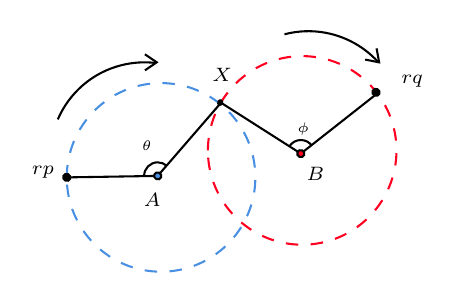
\begin{tikzpicture}[x=0.75pt,y=0.75pt,yscale=-1,xscale=1]
%uncomment if require: \path (0,188); %set diagram left start at 0, and has height of 188

%Straight Lines [id:da6385513002040925] 
\draw    (249.11,107.84) -- (211.13,83.64) ;
%Straight Lines [id:da06022408847837668] 
\draw    (180.14,118.59) -- (209.81,84.31) ;
%Straight Lines [id:da3358007342898651] 
\draw    (136.33,119.3) -- (180.14,118.59) ;
%Straight Lines [id:da6539204452072057] 
\draw    (249.11,107.84) -- (284.68,79.84) ;
%Shape: Ellipse [id:dp6365819441495395] 
\draw  [color={rgb, 255:red, 0; green, 0; blue, 0 }  ,draw opacity=1 ][fill={rgb, 255:red, 74; green, 144; blue, 226 }  ,fill opacity=1 ] (178.53,117.87) .. controls (178.89,117.02) and (179.91,116.65) .. (180.8,117.05) .. controls (181.69,117.45) and (182.12,118.46) .. (181.76,119.3) .. controls (181.4,120.15) and (180.38,120.52) .. (179.49,120.12) .. controls (178.6,119.73) and (178.17,118.72) .. (178.53,117.87) -- cycle ;
%Shape: Ellipse [id:dp49846506020603687] 
\draw  [color={rgb, 255:red, 0; green, 0; blue, 0 }  ,draw opacity=1 ][fill={rgb, 255:red, 255; green, 0; blue, 30 }  ,fill opacity=1 ] (247.49,107.12) .. controls (247.85,106.27) and (248.87,105.91) .. (249.76,106.3) .. controls (250.65,106.7) and (251.08,107.71) .. (250.72,108.56) .. controls (250.36,109.41) and (249.35,109.78) .. (248.45,109.38) .. controls (247.56,108.98) and (247.13,107.97) .. (247.49,107.12) -- cycle ;
%Shape: Circle [id:dp1529302486368378] 
\draw  [color={rgb, 255:red, 74; green, 144; blue, 226 }  ,draw opacity=1 ][dash pattern={on 4.5pt off 4.5pt}] (136.33,119.3) .. controls (136.33,94.21) and (156.67,73.87) .. (181.76,73.87) .. controls (206.85,73.87) and (227.19,94.21) .. (227.19,119.3) .. controls (227.19,144.4) and (206.85,164.74) .. (181.76,164.74) .. controls (156.67,164.74) and (136.33,144.4) .. (136.33,119.3) -- cycle ;
%Shape: Circle [id:dp3970614549640945] 
\draw  [color={rgb, 255:red, 255; green, 0; blue, 32 }  ,draw opacity=1 ][dash pattern={on 4.5pt off 4.5pt}] (204.33,106.3) .. controls (204.33,81.21) and (224.67,60.87) .. (249.76,60.87) .. controls (274.85,60.87) and (295.19,81.21) .. (295.19,106.3) .. controls (295.19,131.4) and (274.85,151.74) .. (249.76,151.74) .. controls (224.67,151.74) and (204.33,131.4) .. (204.33,106.3) -- cycle ;
%Shape: Ellipse [id:dp8019833263877416] 
\draw  [color={rgb, 255:red, 0; green, 0; blue, 0 }  ,draw opacity=1 ][fill={rgb, 255:red, 0; green, 0; blue, 0 }  ,fill opacity=1 ] (209.38,82.86) .. controls (209.63,82.27) and (210.23,81.97) .. (210.71,82.18) .. controls (211.19,82.4) and (211.38,83.05) .. (211.13,83.64) .. controls (210.89,84.22) and (210.29,84.53) .. (209.81,84.31) .. controls (209.32,84.1) and (209.13,83.44) .. (209.38,82.86) -- cycle ;
%Shape: Ellipse [id:dp47771545199155907] 
\draw  [color={rgb, 255:red, 0; green, 0; blue, 0 }  ,draw opacity=1 ][fill={rgb, 255:red, 0; green, 0; blue, 0 }  ,fill opacity=1 ] (134.71,118.59) .. controls (135.07,117.74) and (136.09,117.37) .. (136.98,117.77) .. controls (137.87,118.16) and (138.3,119.17) .. (137.94,120.02) .. controls (137.58,120.87) and (136.57,121.24) .. (135.68,120.84) .. controls (134.78,120.45) and (134.35,119.44) .. (134.71,118.59) -- cycle ;
%Shape: Ellipse [id:dp09642739570555636] 
\draw  [color={rgb, 255:red, 0; green, 0; blue, 0 }  ,draw opacity=1 ][fill={rgb, 255:red, 0; green, 0; blue, 0 }  ,fill opacity=1 ] (283.71,77.59) .. controls (284.07,76.74) and (285.09,76.37) .. (285.98,76.77) .. controls (286.87,77.16) and (287.3,78.17) .. (286.94,79.02) .. controls (286.58,79.87) and (285.57,80.24) .. (284.68,79.84) .. controls (283.78,79.45) and (283.35,78.44) .. (283.71,77.59) -- cycle ;
%Shape: Arc [id:dp7510621770342669] 
\draw  [draw opacity=0] (132.02,91.35) .. controls (137.48,78.7) and (148.6,68.67) .. (163.01,65.16) .. controls (168.32,63.87) and (173.63,63.57) .. (178.76,64.14) -- (173.76,109.3) -- cycle ; \draw  [color={rgb, 255:red, 0; green, 0; blue, 0 }  ,draw opacity=1 ] (132.02,91.35) .. controls (137.48,78.7) and (148.6,68.67) .. (163.01,65.16) .. controls (168.32,63.87) and (173.63,63.57) .. (178.76,64.14) ;  
%Shape: Arc [id:dp018216882026905523] 
\draw  [draw opacity=0] (241.24,50.36) .. controls (251.47,47.67) and (262.68,48.53) .. (272.9,53.58) .. controls (278.03,56.12) and (282.47,59.5) .. (286.14,63.47) -- (252.76,94.3) -- cycle ; \draw  [color={rgb, 255:red, 0; green, 0; blue, 0 }  ,draw opacity=1 ] (241.24,50.36) .. controls (251.47,47.67) and (262.68,48.53) .. (272.9,53.58) .. controls (278.03,56.12) and (282.47,59.5) .. (286.14,63.47) ;  
\draw   (174,60) -- (179.68,63.86) -- (174,67.72) ;
\draw   (285.59,57.13) -- (286.84,63.88) -- (280.1,62.54) ;
%Shape: Arc [id:dp8643721314272893] 
\draw  [draw opacity=0] (173.6,118.63) .. controls (173.6,118.62) and (173.6,118.6) .. (173.6,118.59) .. controls (173.6,114.97) and (176.53,112.04) .. (180.14,112.04) .. controls (181.87,112.04) and (183.44,112.71) .. (184.61,113.8) -- (180.14,118.59) -- cycle ; \draw   (173.6,118.63) .. controls (173.6,118.62) and (173.6,118.6) .. (173.6,118.59) .. controls (173.6,114.97) and (176.53,112.04) .. (180.14,112.04) .. controls (181.87,112.04) and (183.44,112.71) .. (184.61,113.8) ;  
%Shape: Arc [id:dp09604382344880302] 
\draw  [draw opacity=0] (243.68,104.19) .. controls (244.85,102.45) and (246.85,101.3) .. (249.11,101.3) .. controls (251.3,101.3) and (253.24,102.38) .. (254.43,104.03) -- (249.11,107.84) -- cycle ; \draw   (243.68,104.19) .. controls (244.85,102.45) and (246.85,101.3) .. (249.11,101.3) .. controls (251.3,101.3) and (253.24,102.38) .. (254.43,104.03) ;  

% Text Node
\draw (205,65.4) node [anchor=north west][inner sep=0.75pt]  [font=\scriptsize]  {$\vb{X}$};
% Text Node
\draw (172,125.4) node [anchor=north west][inner sep=0.75pt]  [font=\scriptsize]  {$A$};
% Text Node
\draw (250.45,112.78) node [anchor=north west][inner sep=0.75pt]  [font=\scriptsize]  {$B$};
% Text Node
\draw (118,112.4) node [anchor=north west][inner sep=0.75pt]  [font=\scriptsize]  {$\vb{r}\tund{p}$};
% Text Node
\draw (296,68.4) node [anchor=north west][inner sep=0.75pt]  [font=\scriptsize]  {$\vb{r}\tund{q}$};
% Text Node
\draw (171,100.4) node [anchor=north west][inner sep=0.75pt]  [font=\tiny]  {$\theta $};
% Text Node
\draw (246,91.4) node [anchor=north west][inner sep=0.75pt]  [font=\tiny]  {$\phi $};


\end{tikzpicture}

\end{figure}
\noindent
Let the space be $\SM$ and let $A,B\in \SM$ such that about $A,B$ the space is isotropic, that is, any function $\rho(r,\theta,\phi)\equiv \rho(r)$ for  where $r$ is the distance of any point from $A$ or $B$. Let $r\tund{1}, r\tund{2}$ be given such that $r\tund{1}+r\tund{2}>d>|r\tund{1}-r\tund{2}|$ Then effectively we can construct the sets $\mathbb{S}^{d-1}\tund{1}$ and $\mathbb{S}^{d-1}\tund{2}$ where $d$ is the dimension of the space $\SM$
$$\mathbb{S}^{d-1}\tund{1} := \{\vb{x} \in \SM : |\vb{x} - \vb{r}\tund{A}| := r\tund{1}\}\qquad \mathbb{S}^{d-1}\tund{2} = \{\vb{x} \in \SM : |\vb{x} - \vb{r}\tund{B}| = r\tund{2}\}$$
such that $W = \mathbb{S}^{d-1}\tund{1}  \cap \mathbb{S}^{d-1}\tund{2} \neq \emptyset$. Let $\vb{X}\in W$ and consider $\vb{P}\in \mathbb{S}^{d-1}\tund{1},\vb{Q}\in \mathbb{S}^{d-1}\tund{2}$. Since the space is isotropic about point $A$ we can rotate the point $P$ to $X$ about $A$ by an angle $\theta$ such that $\rho$ remains same. 
$$\rho(\vb{P}) = \rho(\vb{X})\equiv \rho(R^A_{\theta}\vb{P}) $$
Now $\vb{X}\in \mathbb{S}^{d-1}\tund{2}$ and since the space is isoptropic about point B, we can rotate it about point $B$ by an angle $\phi$ to $Q$ without changing $\rho$
$$\rho(\vb{X}) = \rho(\vb{Q})\equiv \rho(R^B_\phi \vb{X})$$
Combining the above two expressions we get 
$$\rho(\vb{Q}) = \rho(\vb{P})$$
Since $P$ and $Q$ were arbitrary two points, we can say that $\rho(\vb{x}) = \rho(\vb{y})$ for any $\vb{x}\in \mathbb{S}^{d-1}\tund{1},\vb{y}\in \mathbb{S}^{d-1}\tund{2}$. By varying the radii we can construct different circles that follow this property and thus we get $\rho(\vb{x}) = \rho(\vb{y})\ \forall\ \vb{x}, \vb{y}\in \SM$\\[0.2cm]
\noindent
Thus, isotropy implies homogenity and at large scales, our Universe is both \textit{homogenous} (independent of spatial position) and \textit{isotropic}. \\[0.2cm]
NOTE: Isotropy means that a space looks same in every direction while homogenity means that the space looks the same at every point. If the space was filled with some parallel strings, then the space would have been homogenous but not isoptropic, since depending on the orientations of the strings, the space would look different in different directions.\\[0.2cm] Now, another interesting question, is our Universe finite or infinite? And does this even matter? \\[0.2cm]
This question is contained in the list of \textit{fourteen unanswered questions} which Gautam Buddha refused to answer, stating that these kind of questions prevents us from liberation. And this question really doesn't matter that much. 
\subsection{Olber's Paradox}
\begin{center}
    "The night sky should be bright!"
\end{center}
Consider a star at a distance $r$ and of absolute luminosity $L$. Then the apparent luminosity of the star for an observer at the origin is $$A(r) = \frac{L}{4\pi r^2}$$
Let the number density of the star at a distance $r$ be $n(r)$. Then the apparent luminosity of the whole sky as viewed by the observer for the stars present between $r$ and $r+\dd r$ is 
$$\dd E = (4\pi r^2 \dd r) n(r) A(r)$$
Then the total observed luminosity by the observer 
$$E =\int \dd E = \int\limits_0^\infty n(r)L\ \dd r \xrightarrow[\text{Universe}]{\text{homogenous}}   n\tund{0} L\int\limits_0^\infty \dd r \rightarrow \infty$$
Clearly this integral diverges and the observed luminosity is apparently infinite which tells us that the night sky should be bright if the observed luminosity (brightness) diverges which is clearly a contradiction. The divergence came because we carried out the integration till \textit{infinity}. There might be some issue with this then and we infer that either  \\[0.2cm]
$\vartriangleright \ \text{The Universe is finite in age}$
\begin{center}
    \large \textbf{OR}
\end{center}
$\vartriangleright \ \text{Light can reach to us only from a finite, restricted part of the Universe}$\\[0.2cm]
Modern models estimate that indeed Universe has a finite age and thus, we can in principle detect only objects which are situated as far light-years as the age of the Universe and we anything beyond that is out of our reach. 
